\documentclass[english]{report}
\usepackage[T1]{fontenc}
\usepackage[latin9]{inputenc}
\usepackage{geometry}
\geometry{verbose,tmargin=2.54cm,bmargin=2.54cm,lmargin=2.54cm,rmargin=2.54cm}
\usepackage{float}
\usepackage{graphicx}
\graphicspath{{../images/}}
\usepackage{siunitx}
\usepackage{babel}
\usepackage{booktabs}
\usepackage[toc,page]{appendix}


\makeatletter
\usepackage{multicol}
\makeatother

\setcounter{secnumdepth}{0}


\title{Project CODENAME}
\author{Joshua Morin-Baxter}
\date{\today}


\begin{document}

\newcommand{\amountofheliumtobeused}{142 }

\maketitle

\tableofcontents


\part{Introduction}

\begin{appendix}
  \addcontentsline{toc}{section}{List of Figures}
  \listoffigures
  \addcontentsline{toc}{section}{List of Tables}
  \listoftables
\end{appendix}

\newpage

\section{4th Annual High Altitude Challenge}
This document is an overview of a design concept submitted to the
4th Annual High Altitude Challenge at Stevens High School. The competition
challenged over 30 teams to submit a grant proposal for a high altitude
balloon payload. This payload will be attached to a helium propelled weather balloon and lifted off into the atmosphere, to a projected height of over 120,000ft.  The payload must then return to the ground safely (via parachute.)  The exact function of the payload is typically left up to individual teams, but general guidelines include taking sensor readings of the atmosphere and/or aerial photographs.  The more specific guidelines put in place for this year's competition are described below:

The payload is required to\dots
\begin{enumerate}
\item Adhere to all federal, state, and local laws and comply with FCC and
FAA regulations.
\item Communicate with the ground at all times via APRS radio.\label{req:APRS}
\item Include a redundant means of locating the payload on the ground, should the primary method fail.\label{req:redundant_location}
\item Return photographic evidence of the entire flight, including the balloon
burst.
\item Measure external temperature and pressure AND monitor internal temperature
and pressure at all times during the flight\label{req:sensors} of the High Altitude Challenge.
\item Survive 10-g accelerations in every orientation.
\item Be Reusable.
\item Measure 3-Axis Acceleration.\label{req:accelerometer}
\item Weigh LESS THAN 250 grams (including parachute and lines).
\item Minimize instabilities (specifically spinning.)\label{req:spinning}
\end{enumerate}
The payload designed by Team CODENAME won first place in the competition
and was awarded a \$3,000 grant to build the payload according to the specifications described in this document.


\section{Component Summary}
%TODO change this page to reflect what was actually launched
\begin{figure}[H]
\begin{centering}
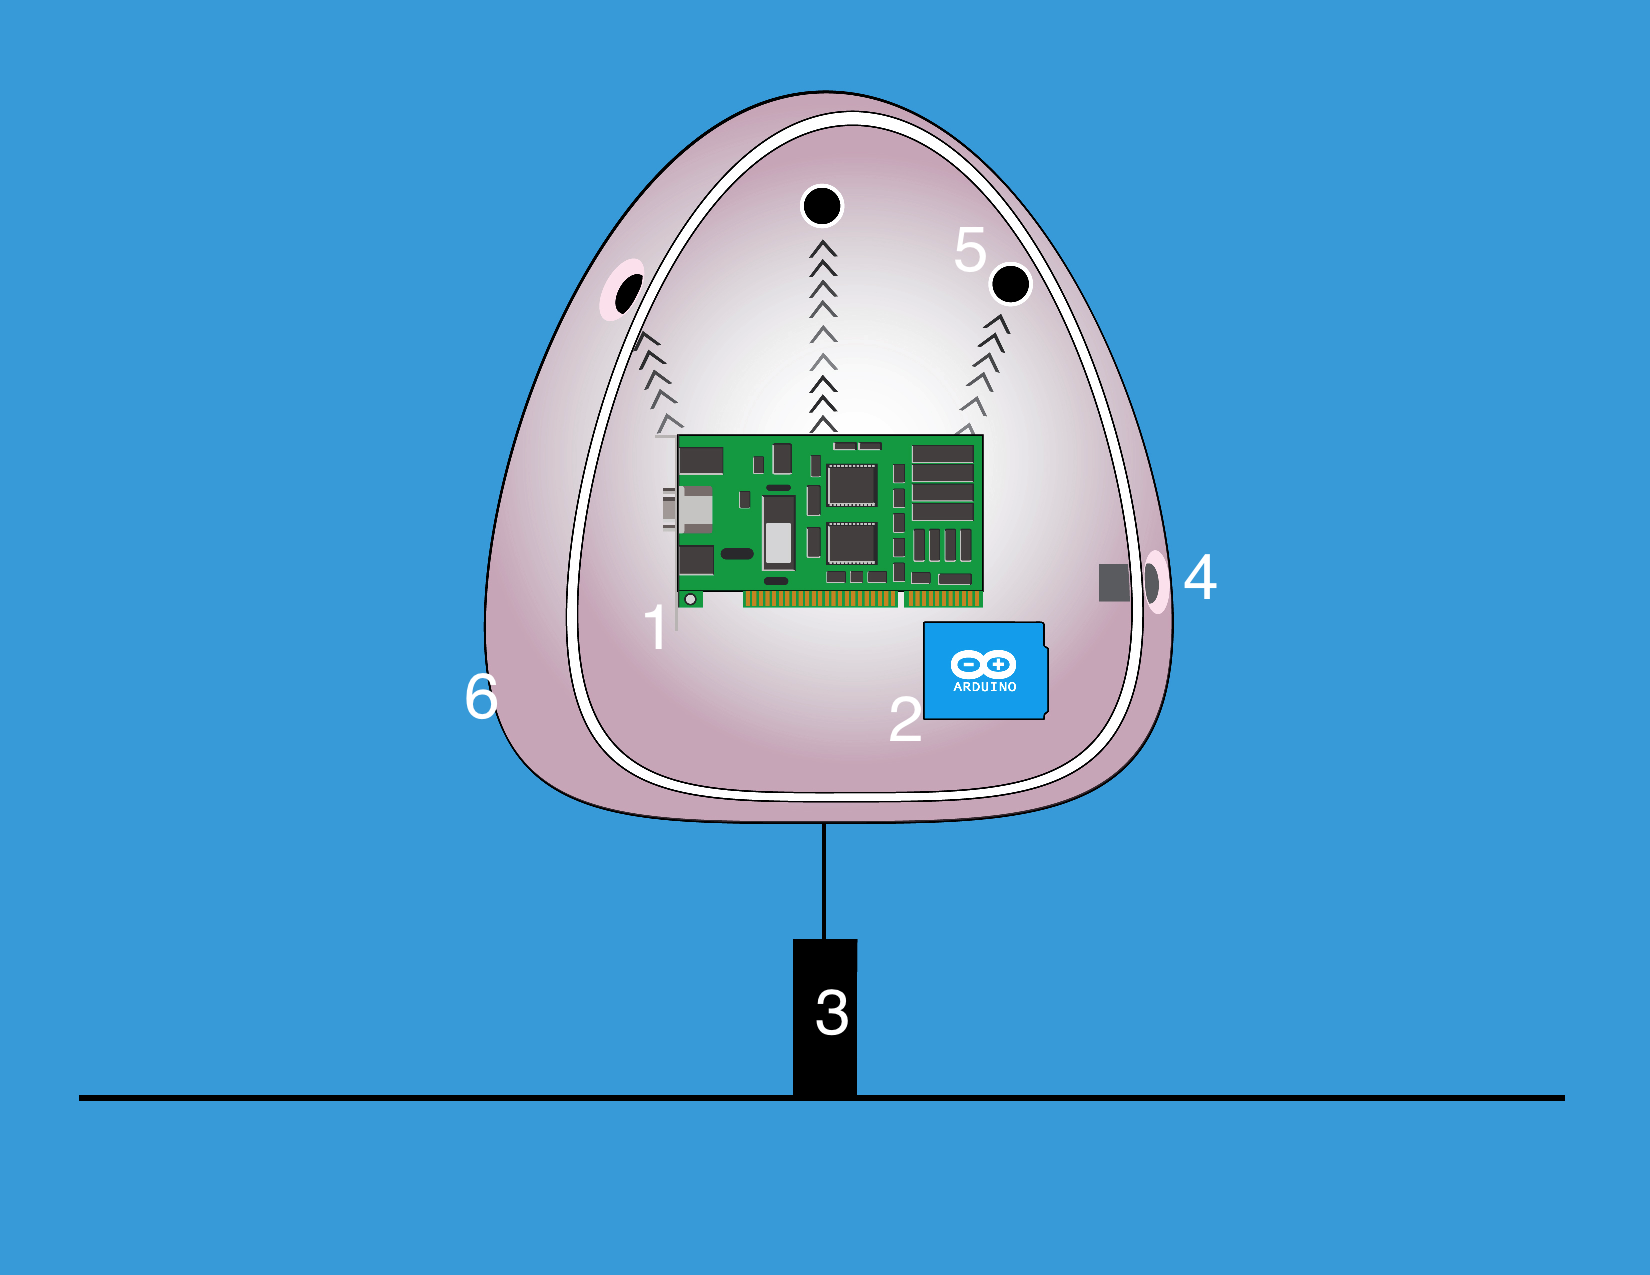
\includegraphics[scale=0.3]{./images/karah_physics_2-1}
\par\end{centering}
\caption{Cross-section of payload}
\end{figure}

\begin{multicols}{2}
\begin{enumerate}
\item \textbf{Samsung Galaxy S4 Chipset} Stripped-down computer board taken
from phone and reprogrammed.  Contains majority of payload's sensors and stores all payload sensor data in internal storage. Eight hour projected battery life.
\item \textbf{Arduino Micro} Provides an interface between the Tracksoar and the Samsung Galaxy S4 Chipset, as well as collecting data from the payload's ozone sensor.
\item \textbf{Tracksoar APRS Transmitter} Leverages existing radio relays
to keep payload in constant contact after takeoff; sends all sensor
data to ground station in real-time.  Also equipped with GPS
capable of high altitude positioning, along with external temperature
and pressure sensors. Twelve hour projected battery life, does not require other computing components to function.
\item \textbf{External Cameras} 2MP and 15MP photographs taken for the duration
of the flight.
\item \textbf{Additional Sensors} Sixteen distinct sensors (only three diagrammed here).  These are discussed further further in Part \ref{internal_components}.
\item \textbf{Foamular 150} Insulating outer shell.  Lightweight and impact resistant.
\end{enumerate}
\end{multicols}
Not pictured: Parachute and balloon.

\pagebreak
\section{Flight Path}
\label{ground-station}
%TODO this entire part needs to be overhauled to include our use of the spreadsheets
%TODO it also needs to delicately discuss how crappy our balloon performed and how badly we predicted everything
The target landing area for the payload is the Badlands National Park; the launch window will open in the first weeks of April, 2017, due to weather concerns.  Project CODENAME will use the HabHub\cite{HabHub} predictive engine to determine more exact launch times.  This predictive engine provides accurate predictions of likely flight paths up to 180 hours into the future. The following variables are required to generate accurate predictions:

\begin{description}

\item [Launch Point (lat long)] 44.075604, -103.286696 (Stevens High School Football Field)
\item [Launch Point Elevation] 1043.2 m or 3422.5 feet
\item [Burst Altitude] 39060m*
\item [Ascent Rate] $3.83 \si{\frac{m}{s}}$*
\item [Descent Rate] $4.5658\si{\frac{m}{s}}$*
\end{description}
*Determined by helium volume and balloon size, positive lift, and parachute size, respectively.  These items are discussed in depth in Part \ref{part:external}.

\begin{figure}[H]
\begin{centering}
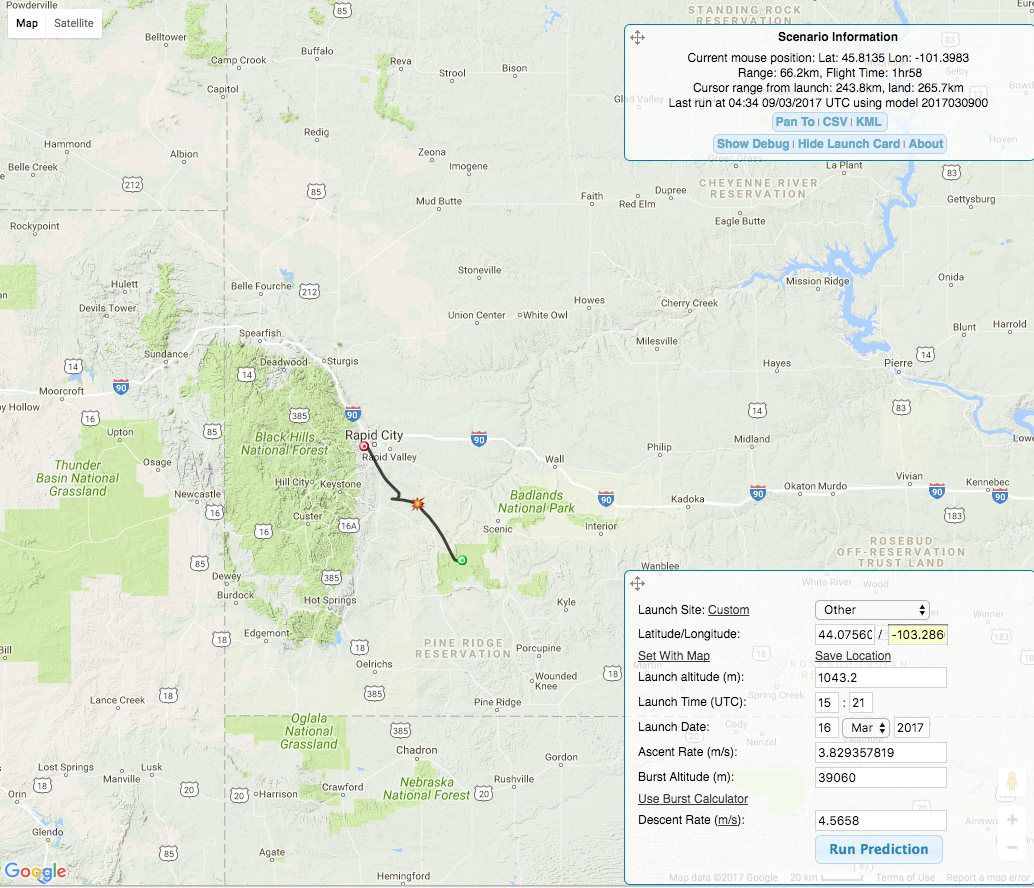
\includegraphics[scale=0.4]{./images/habhub}
\par\end{centering}
\caption{Example HabHub flight path prediction map for March 18, 2017.}
\end{figure}



\part{Internal Components and Software}
\label{internal_components}

Project CODENAME has developed two important operational scripts: one runs on the S4 Chipset and is essentially a highly persistent app that commandeers the phone's onboard sensors and camera; the second is a modification to the source code shipped with the Tracksoar APRS Tracking device.  These are discussed in greater detail within subsequent sections.


\section{Samsung Galaxy S4 Chipset}

This is the primary computing component of the payload. It consists
of a computer board taken from a Samsung Galaxy S4 phone, reprogrammed
to suit the needs of the project. The chipset contains eight integrated
sensors, including a RGB light sensor, a magnetometer, a gravimeter,
an accelerometer, thermometer, barometer, hygrometer, and sensors
to measure orientation vectors. Since all of these sensors are built into
the chipset, they add no extra weight and write data directly to the
phone's memory where it can be stored for later retrieval. Additionally,
the two chipset cameras (the front-facing and rear-facing cameras
of the S4 phone, 2MP and 13MP respectively) provide two unique angles
from which the payload can take photographs for the duration of the
flight. These cameras are removed from the board and reattached with
longer wires to optimize their viewing positions. All sensor data
collected by the other two computing components (described below)
are written to the S4's internal storage, which can be read after
the payload returns to the ground.  An extended lithium-ion battery (5200mAh) provides a projected eight hours of battery life under ideal operating conditions.

The script roots the S4 chipset to maximize utility, reduce unwanted phone operations and increase battery life. %TODO write more in-depth on the significance and importance of the operational script

\begin{figure}[H]
\begin{centering}
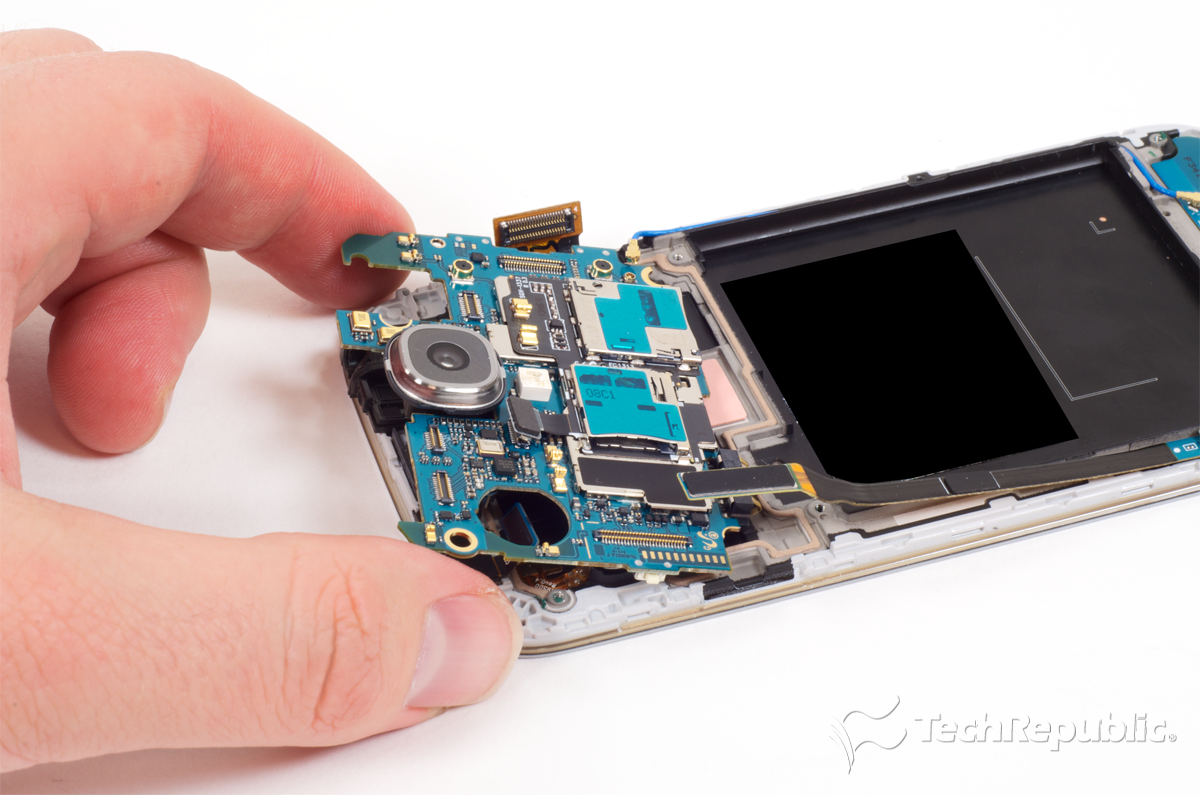
\includegraphics[scale=0.2]{./images/chipset}
\par\end{centering}
\caption{A Samsung Galaxy S4 Chipset being removed from the rest of the phone.}
\end{figure}


\section{Tracksoar APRS Transmitter}

The Tracksoar APRS transmitter is the third and final computing component
aboard the payload. While it is equipped with several sensors (specifically
a GPS sensor along with external temperature, pressure, and humidity)
it primarily serves as the point of contact between the payload and
the ground. The transmitter transmits the payload's location (and
its sensor readings) on the 2 meter band, where it is picked up by
the APRS relay system and can be received anywhere in the state of
South Dakota, as per requirement \ref{req:APRS}. This allows for constant monitoring of the payload's
position and exact conditions. The Tracksoar also has an independent
power source projected to last up to 12 hours; this ensure that even
if the rest of the payload loses power the capsule will continue transmitting
its location.  The Tracksoar is connected to the Arduino micro via the I$^2$C port.

\begin{figure}[H]
\begin{centering}
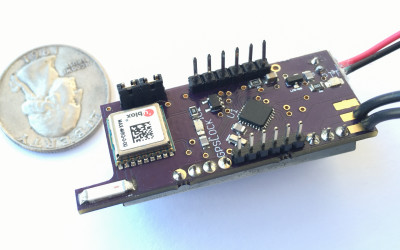
\includegraphics{./images/tracksoar}
\par\end{centering}
\caption{A Tracksoar APRS Tracking Device shown alongside quarter for scale. Antenna and battery not pictured.}
\end{figure}


\pagebreak
\section{Sensors}

While the High Altitude Challenge requires only four sensors (internal
and external temperature and pressure), the project CODENAME payload
is equipped with a total of 16 distinct sensors distributed among
the two computing components described above. This section examines
the purpose of each sensor or sensor group.  In this discussion they have been loosely grouped into two categories
as shown below\@.

\subsubsection*{Category 1}

Sensors relating to the management and operation of the payload itself.
\begin{itemize}
\item \textbf{GPS (latitude and longitude) and altimeter: }These sensors
provide the payload's exact position. This is the data used by the
ground station to track the payload's flight path.
\item \textbf{Accelerometer and orientation vector sensors: }These sensors
allow the payload to determine its exact orientation at all times;
the data can be used to recreate how the payload is turning or spinning
in the air. It also improves location accuracy as it can be used to
measure payload flight trajectory over short distances between GPS
measurements.  The accelerometer also meets requirement \ref{req:accelerometer} of the High Altitude Challenge.
\item \textbf{Internal thermometer, internal barometer and internal hygrometer:}
Measures the ambient temperature, pressure, and humidity, respectively,
on the inside of the payload. This provides important data on the
internal operating conditions of the payload, as per requirement~\ref{req:sensors} of the High Altitude Challenge.
\end{itemize}

\subsubsection*{Category 2}

Sensors relating to to the capture of unique scientific data.
\begin{itemize}
\item \textbf{External thermometer, external barometer, and external hygrometer:
}Measures the ambient temperature, pressure, and humidity, respectively,
on the outside of the payload. This data provides information on atmospheric
conditions around the payload,~\ref{req:sensors} of the High Altitude Challenge.
\item \textbf{Gravimeter: }Measures strength of earth's gravitational field
at a given altitude.
\item \textbf{Magnetometer: }Measures strength of earth's magnetic field
at a given altitude.
\end{itemize}


\begin{figure}[H]
\begin{centering}
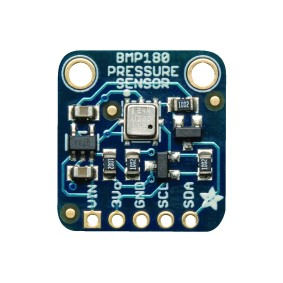
\includegraphics{./images/bmp}
\par\end{centering}
\caption{BMP-180 Sensor used by Tracksoar to measure temperature and pressure.}
% TODO determine if this is the right sensor and what it did
\end{figure}

% TODO add data tables including the data collected by all these sensors


\part{External}
\label{part:external}

\section{Housing}

The payload shape was inspired by the famous Soyuz capsule, first
employed by the USSR and NASA as early as 1960 but still in use today.  This shape is ideal for stabilizing a craft as it reenters the atmosphere (requirement number \ref{req:spinning} of the High Altitude Challenge requirements.)  This proved particularly relevant for the payload as the parachute did not deploy.

%TODO confirm this is actually Foamular 150
The housing material is Foamular 150.  This is an insulating foam that is ideal for keeping the payload within operating temperature conditions, without adding unnecessary weight.

\begin{figure}[H]
\begin{centering}
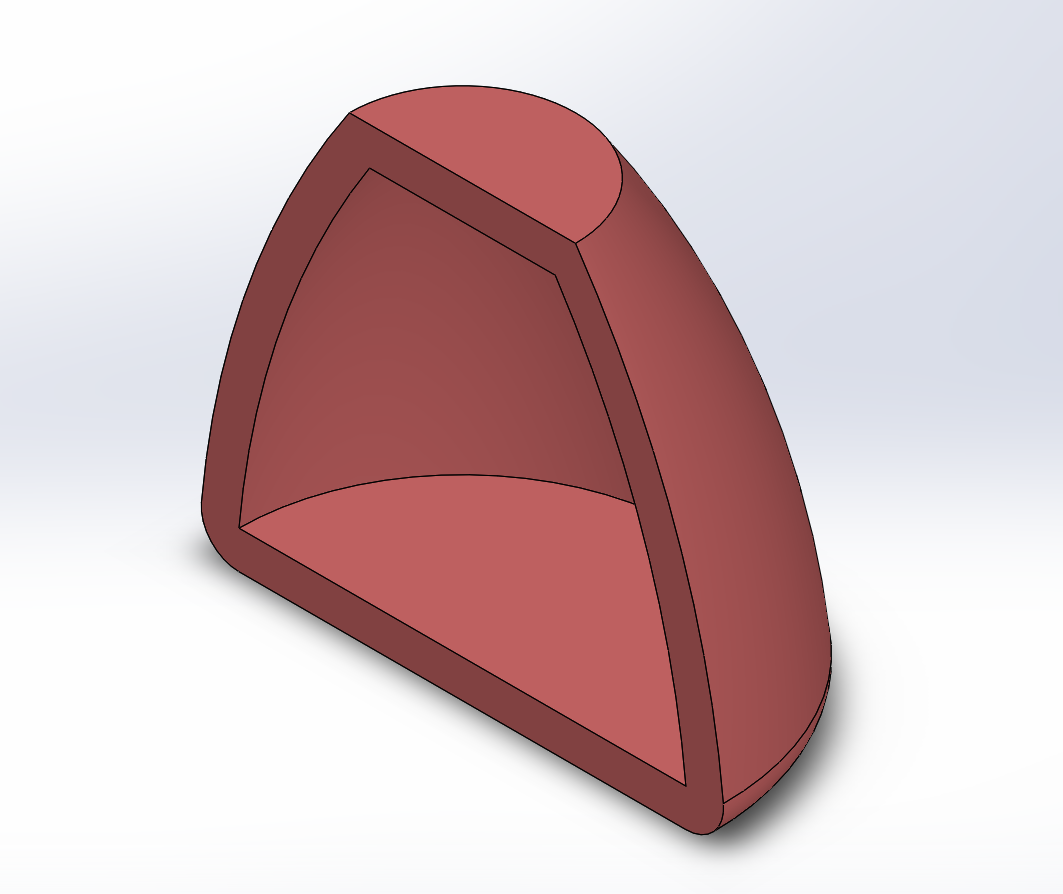
\includegraphics[scale=0.5]{./images/shape}
\par\end{centering}
\caption{Rendering of Payload External Shape}

\end{figure}

%TODO add an explanation of how exactly Nate machined the payload to be the beautiful work of art it is

\newpage
\section{Balloon and Helium}
Past teams in the High Altitude Challenge have typically used 1200 gram weather balloons; however, Project CODENAME has selected a larger 1500 gram weather balloon.  This increase in size will allow the payload to travel higher in a shorter amount of time, though it will increase the helium demand.  See Table \ref{balloon_size} in the appendix for a comparison of the standard weather balloon sizes\cite{balloon-performance-calculator}.


Calculations determined that the  amount of positive lift needed for the payload to achieve the best possible combination of flight time and burst altitude was approximately 160 grams.  A dummy payload was created weighing 410 grams (250+160); this was attached to the balloon as it was filled, and fill stopped when the balloon became buoyant.  Sponsor A\&B Welding of Rapid City donated the helium required for the flight.
% what calculations

Given any one type of balloon, the exact amount of helium that is needed comes from a consideration of two factors: burst altitude and flight time.  As more helium is added to the balloon, flight time decreases (which is an important consideration for the battery life of the payload) but burst altitude also decreases. Conversely, less helium ensures a higher burst altitude, but a longer flight time.  These relationships are demonstrated in Figure~\ref{fig:heliumgraph}.

\begin{figure}[H]
\begin{centering}
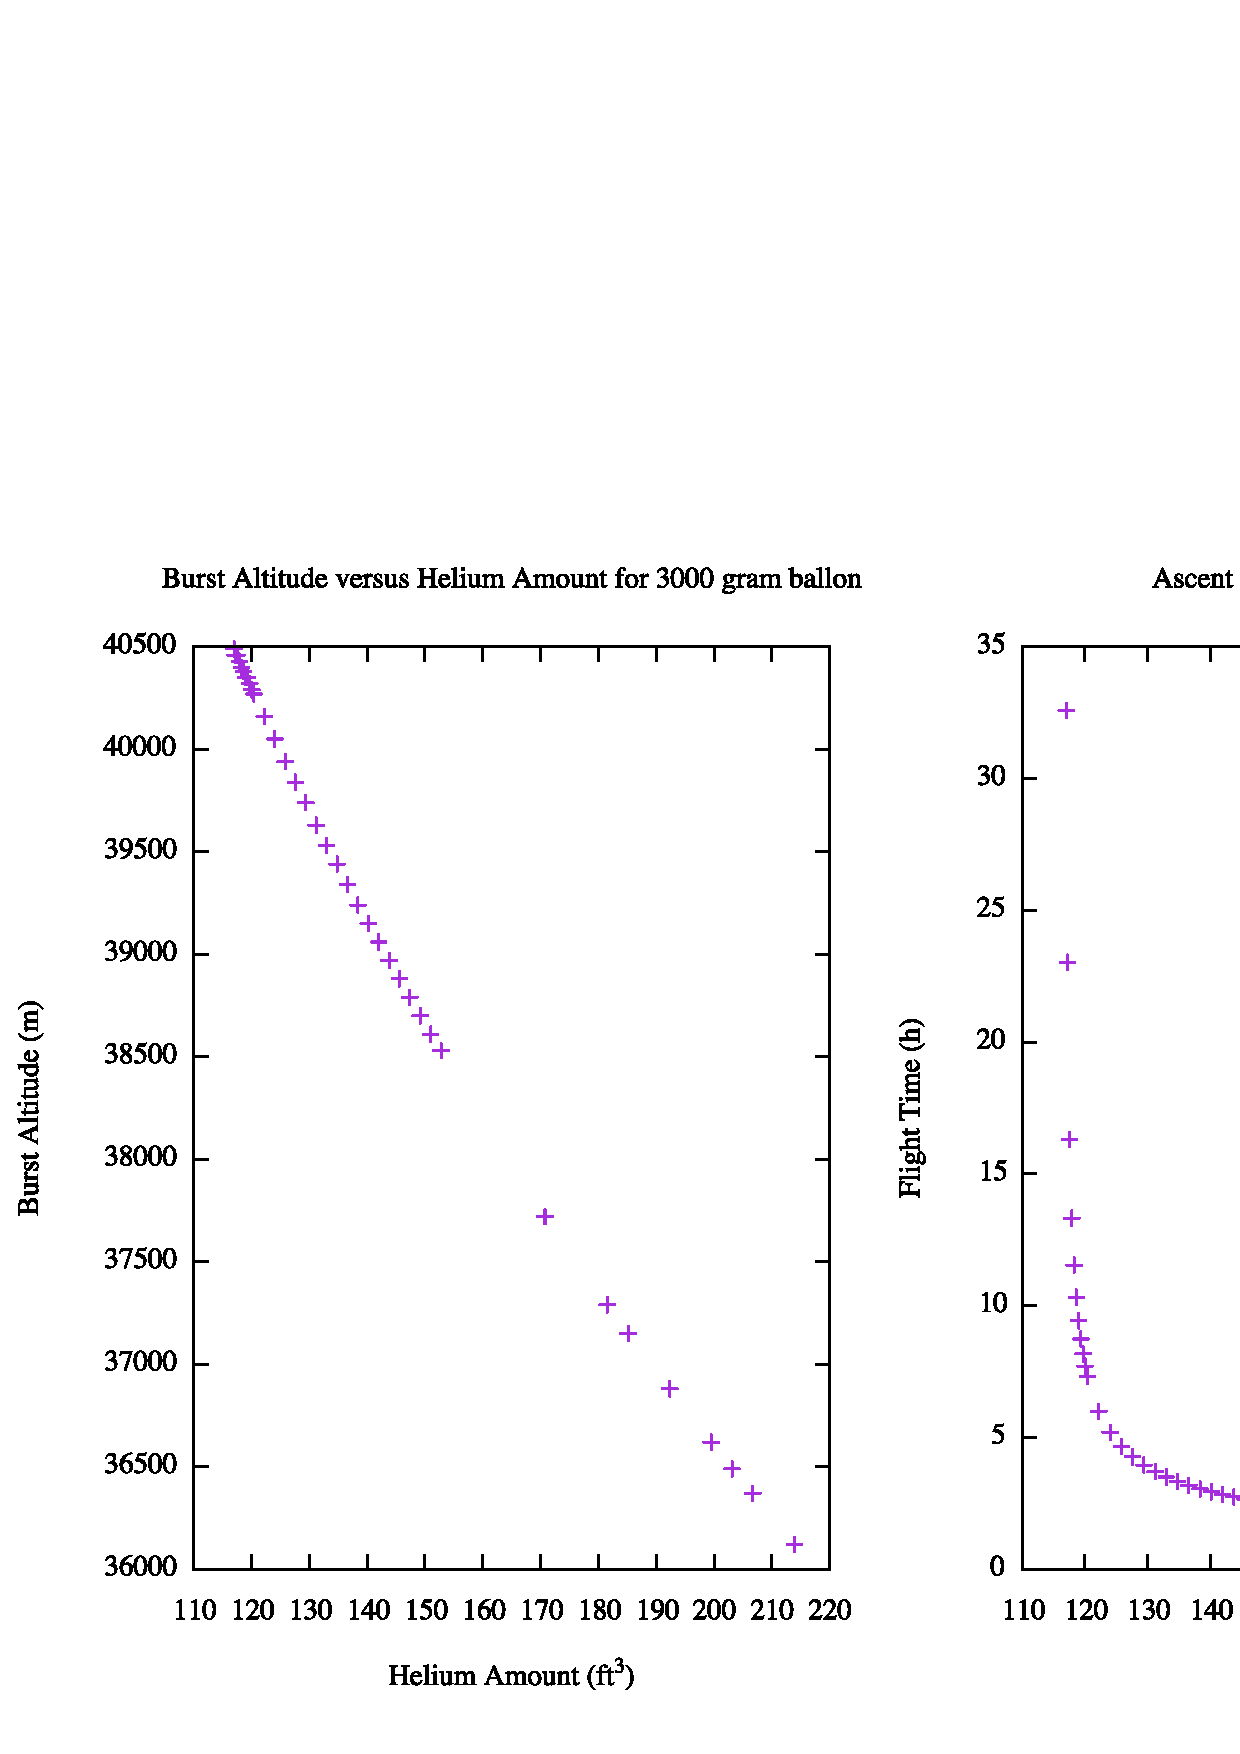
\includegraphics[scale=0.5]{./graphs/heliumgraph}
\par\end{centering}
\caption{Graphs of ascent time and burst altitude, respectively, versus amount of helium.}
\label{fig:heliumgraph}
\end{figure}


\newpage
\section{Parachute}
\label{sec:parachute}
The following equation\cite{parachute-equation} is often used to calculate the necessary parachute diameter to land a payload at a given speed.
\begin{equation}
d = \sqrt{\frac{8mg}{\pi rC_dv^2}}
\label{eq:parachute_original}
\end{equation}
Where
\begin{description}
  \item $d$ = diameter of the parachute
  \item $m$ = mass of payload
  \item $r$ = $1.22\si{\frac{kg}{m^3}}$ (density of air)
  \item $C_d$ = 1.5 (the drag coefficient for a true, dome shaped parachute)
  \item v = velocity at time of impact with ground
\end{description}

Research\cite{3to5} suggested that payload's impact-resistant shell would allow it to land at speeds between 3\si{\frac{m}{s}} and $5\si{\frac{m}{s}}$ without sustaining major internal damage.  Solving equation \ref{eq:parachute_original} for each of these velocities provides the range for the ideal diameter of Project CODENAME's parachute (assuming mass to be 250 grams).

\begin{equation}
d = \sqrt{\frac{8\cdot 0.25\si{kg} \cdot 9.81\si{\frac{m}{s}}}{\pi \cdot 1.22\si{\frac{kg}{m^3}}\cdot1.5 \cdot 3^2}}
\end{equation}

\begin{equation}
d = 0.616\si{m}
\label{d_upper}
\end{equation}


\begin{equation}
d = \sqrt{\frac{8\cdot 0.25\si{kg} \cdot 9.81\si{\frac{m}{s}}}{\pi \cdot 1.22\si{\frac{kg}{m^3}}\cdot1.5 \cdot 5^2}}
\end{equation}

\begin{equation}
d = 0.369\si{m}
\label{d_lower}
\end{equation}

  Equations \ref{d_lower} and \ref{d_upper} suggest that the optimum parachute diameter is between 0.369m and 0.616m. Based on these figures, Project CODENAME selected the TARC-16 Parachute to accompany the payload into orbit.  This parachute has a diameter of 0.4064m (16"), which provides a descent rate of $4.5658\si{\frac{m}{s}}$ according to equation
\ref{eq:parachute_original}.

The parachute was tested in a droptest from the Stevens High School auditorium catwalk.  A dummy payload was fastened to the parachute (approximating the weight of the actual payload) and it was filmed as it fell 34 feet to the ground.  The freeware program Tracker (available at http://physlets.org/tracker/) was used to analyze the distance the parachute fell with respect to time over the last 12 feet of the fall.  The resulting position-time graph is displayed in Figure \ref{fig:parachute-derivative}.  Since the slope is a constant 1.426\si{\frac{m}{s}}, this was taken to be the terminal velocity of the parachute. % figure out what went wrong here

Unfortunately, during the flight of Project CODENAME, the parachute never deployed.  This was a result of the remnants of the balloon becoming entangled in the lines of the parachute on its descent.  Luckily, the payload landed entirely intact with only minor external damage.

%TODO add the actual terminal velocity the payload achieved

\begin{figure}
\begin{centering}
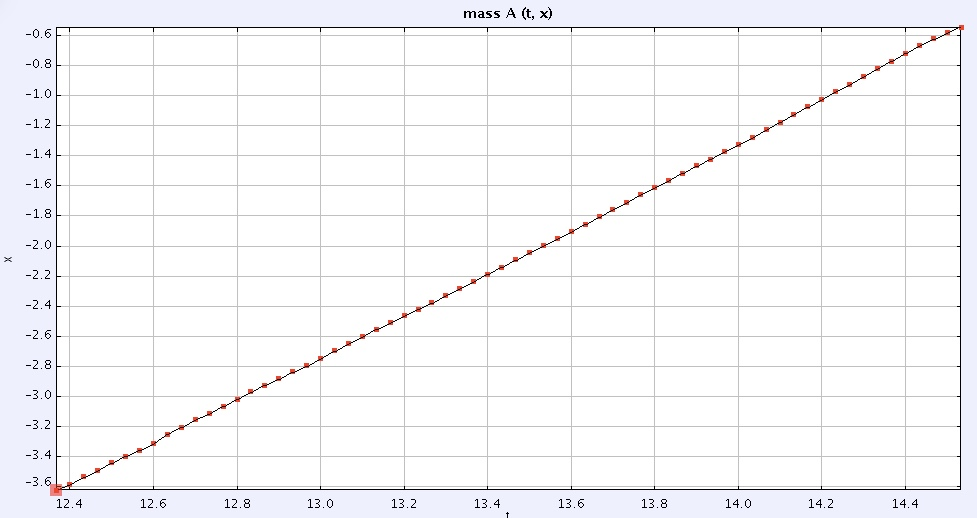
\includegraphics{./graphs/parachute-derivative}
\par\end{centering}
\caption{Position-time graph showing terminal velocity of TARC-16 parachute and dummy payload.}
\label{fig:parachute-derivative}
\end{figure}

The outside of the parachute was painted in phosphorescent paint; This increased the visibility of the payload on the ground during a night search, providing a secondary method for locating it after descent as per requirement \ref{req:redundant_location} of the High Altitude Challenge.


\part{Data Collected}

This is a discussion of the data collected by the chipset and the Tracksoar from launch to landing.

%TODO expand this a lot - it is probably the most important section





\begin{thebibliography}{9}
  %TODO fix citation issues...ask Dr. Smith

\bibitem{HabHub}
HabHub Predictive Engine
\\\texttt{http://predict.habhub.org/}

\bibitem{balloon-performance-calculator}
Balloon Performance Calculator
\\\texttt{http://tools.highaltitudescience.com/}

\bibitem{parachute-equation}
Parachute Descent Calculations
\\\texttt{http://www.rocketmime.com/rockets/descent.html}

\bibitem{3to5}
Shell Impact Resistance
\\\texttt{http://www.rocketmime.com/rockets/descent.html}
\end{thebibliography}


\begin{appendices}
  \chapter{Table Data}
  \begin{table}[]
  \centering
  \label{balloon_size}
  \begin{tabular}{@{}llllll@{}}
  \toprule
  \textbf{Positive Lift (g)} & \textbf{Balloon Size (g)} & \textbf{He ($ft^3$)} & \textbf{Burst Height (m)} & \textbf{Ascent Rate $\si{\frac{m}{s}}$} & \textbf{Time (h)} \\ \midrule
  \multicolumn{1}{|l|}{500} & \multicolumn{1}{l|}{600} & \multicolumn{1}{l|}{48.53} & \multicolumn{1}{l|}{31330} & \multicolumn{1}{l|}{4.63} & \multicolumn{1}{l|}{1.88} \\ \midrule
  \multicolumn{1}{|l|}{500} & \multicolumn{1}{l|}{1200} & \multicolumn{1}{l|}{70.10} & \multicolumn{1}{l|}{35190} & \multicolumn{1}{l|}{4.09} & \multicolumn{1}{l|}{2.39} \\ \midrule
  \multicolumn{1}{|l|}{500} & \multicolumn{1}{l|}{1500} & \multicolumn{1}{l|}{80.89} & \multicolumn{1}{l|}{36650} & \multicolumn{1}{l|}{3.90} & \multicolumn{1}{l|}{2.61} \\ \midrule
  \multicolumn{1}{|l|}{500} & \multicolumn{1}{l|}{3000} & \multicolumn{1}{l|}{134.81} & \multicolumn{1}{l|}{39440} & \multicolumn{1}{l|}{3.29} & \multicolumn{1}{l|}{3.33} \\ \midrule
  \multicolumn{1}{|l|}{1000} & \multicolumn{1}{l|}{600} & \multicolumn{1}{l|}{66.51} & \multicolumn{1}{l|}{29230} & \multicolumn{1}{l|}{5.89} & \multicolumn{1}{l|}{1.38} \\ \midrule
  \multicolumn{1}{|l|}{1000} & \multicolumn{1}{l|}{1200} & \multicolumn{1}{l|}{88.08} & \multicolumn{1}{l|}{33620} & \multicolumn{1}{l|}{5.37} & \multicolumn{1}{l|}{1.74} \\ \midrule
  \multicolumn{1}{|l|}{1000} & \multicolumn{1}{l|}{1500} & \multicolumn{1}{l|}{98.86} & \multicolumn{1}{l|}{35240} & \multicolumn{1}{l|}{5.16} & \multicolumn{1}{l|}{1.90} \\ \midrule
  \multicolumn{1}{|l|}{1000} & \multicolumn{1}{l|}{3000} & \multicolumn{1}{l|}{152.79} & \multicolumn{1}{l|}{38530} & \multicolumn{1}{l|}{4.47} & \multicolumn{1}{l|}{2.40} \\ \midrule
  \multicolumn{1}{|l|}{2000} & \multicolumn{1}{l|}{600} & \multicolumn{1}{l|}{102.46} & \multicolumn{1}{l|}{26390} & \multicolumn{1}{l|}{7.22} & \multicolumn{1}{l|}{1.02} \\ \midrule
  \multicolumn{1}{|l|}{2000} & \multicolumn{1}{l|}{1200} & \multicolumn{1}{l|}{124.03} & \multicolumn{1}{l|}{31310} & \multicolumn{1}{l|}{6.77} & \multicolumn{1}{l|}{1.28} \\ \midrule
  \multicolumn{1}{|l|}{2000} & \multicolumn{1}{l|}{1500} & \multicolumn{1}{l|}{134.81} & \multicolumn{1}{l|}{33100} & \multicolumn{1}{l|}{6.59} & \multicolumn{1}{l|}{1.40} \\ \midrule
  2000 & 3000 & 188.74 & 37010 & 5.89 & 1.75 \\ \bottomrule
  \end{tabular}
  \caption{Comparison of Balloon Size for a given amount of positive lift}
  \end{table}
\end{appendices}

\begin{table}[H]
\begin{raggedright}
\begin{tabular}{|l|l|r|r|}
\hline
\textbf{Item Number} & \textbf{Component} & \textbf{Cost (USD)} & \textbf{Weight (grams)}\tabularnewline
\hline
\hline
ASIN: B00O2ALRNS & Samsung Galaxy S4 (SGH-I337, 16 GB) & 100.86 & 25.00\tabularnewline
\hline
-{}- & Camera Connection Cord(x2) & -{}- & 2.00\tabularnewline
\hline
ASIN: B00S4FCLJ6 & Chipset Battery & 12.99 & 50.00\tabularnewline
\hline
SKU: 0001 & Tracksoar & 195.00 & 40.00\tabularnewline
\hline
-{}- & Tracksoar-Arduino cables & -{}- & 4.00\tabularnewline
\hline
SKU: 0007 & Tracksoar Programming shield & 35.00 & 0.00\tabularnewline
\hline
a000053 & Arduino Interface & 24.95 & 13.00\tabularnewline
\hline
UPC: 65030863186 & Phone-Arduino cord & 6.99 & 8.00\tabularnewline
\hline
UPC:6955170849291 & SainSmart MQ131 Ozone Sensor & 23.98 & 8.50\tabularnewline
\hline
SKU: 1631286 & Foamular Sheets (Housing) & 51.29 & 13.00\tabularnewline
\hline
none, Model: TARC-16 & Parachute & 27.00 & 35.00\tabularnewline
\hline
-{}- & Fishing Swivel \& Kite String & -{}- & 0.30\tabularnewline
\hline
WS2812B & 3 LED LIGHT (Breakout WS2812B) & 8.85 & 4.08\tabularnewline
\hline
ASIN: B0007CM6GW & Photographic Film (Fuji Natura 1600 135-36) & 16.47 & 2.00\tabularnewline
\hline
\textbf{Total} &  & \textbf{503.38} & \textbf{204.88}\tabularnewline
\hline
\end{tabular}
\par\end{raggedright}
\caption{Cost and weight data for Project CODENAME.}

\end{table}

\chapter{Tracksoar Data}
\label{tracksoar-data}


\begin{figure}[H]
\begin{centering}
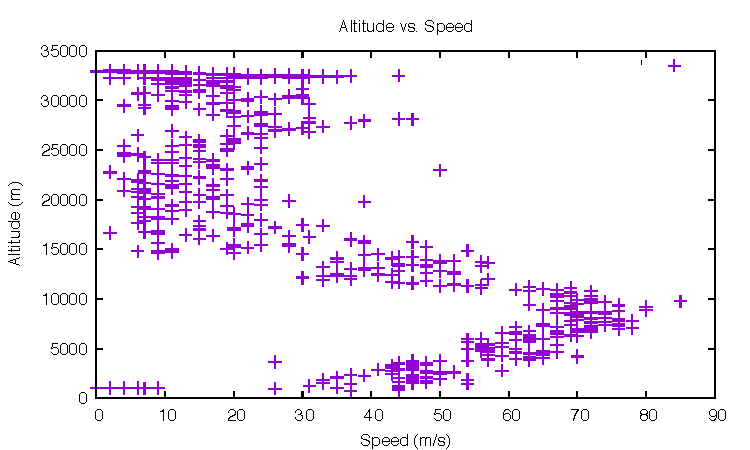
\includegraphics{./tracksoar/altitude-speed}
\par\end{centering}
\caption{}
\label{ts:altitude-speed}
\end{figure}

\begin{figure}[H]
\begin{centering}
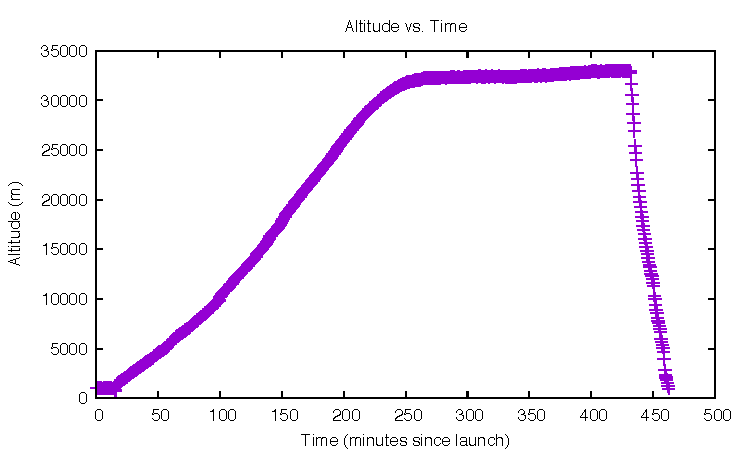
\includegraphics{./tracksoar/altitude-time}
\par\end{centering}
\caption{}
\label{ts:altitude-time}
\end{figure}

\begin{figure}[H]
\begin{centering}
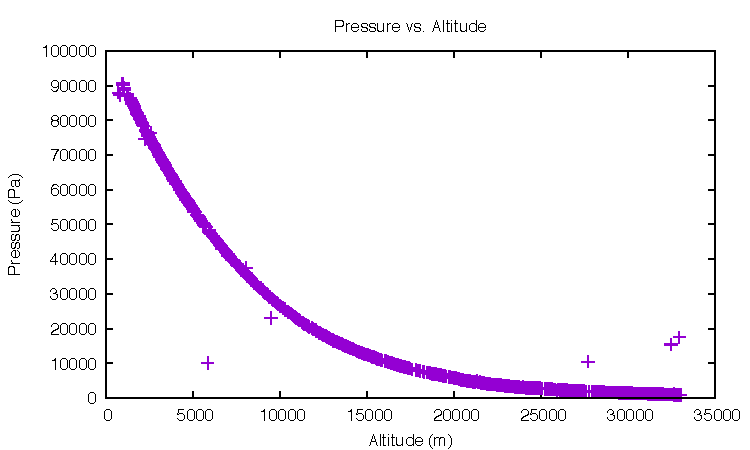
\includegraphics{./tracksoar/pressure-altitude}
\par\end{centering}
\caption{}
\label{ts:pressure-altitude}
\end{figure}

\begin{figure}[H]
\begin{centering}
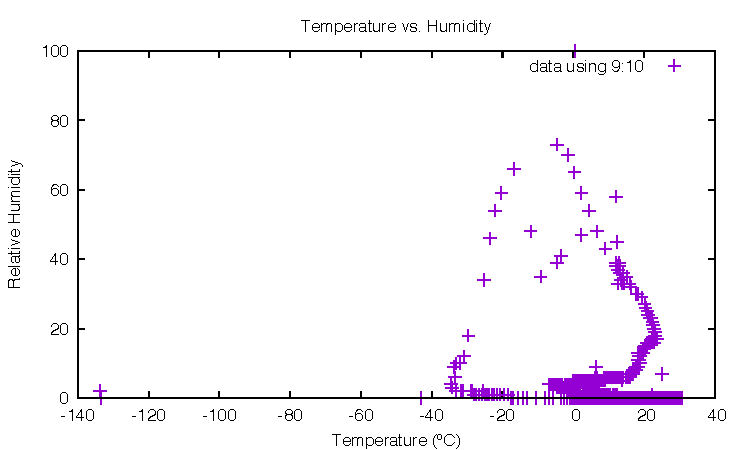
\includegraphics{./tracksoar/rh-temp}
\par\end{centering}
\caption{}
\label{ts:rh-temp}
\end{figure}

\begin{figure}[H]
\begin{centering}
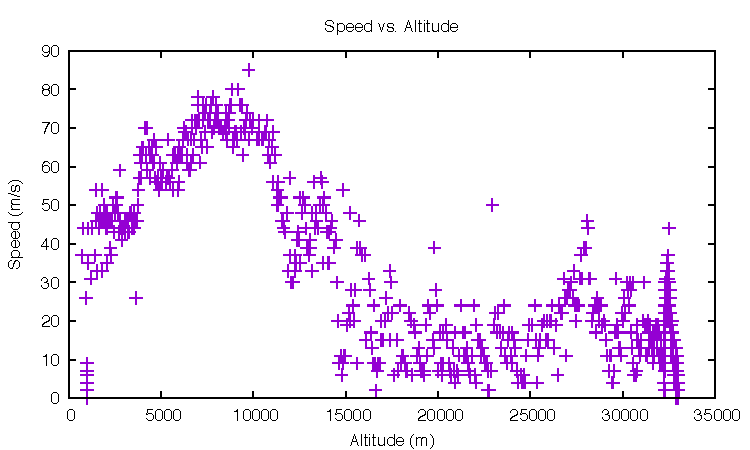
\includegraphics{./tracksoar/speed-altitude}
\par\end{centering}
\caption{}
\label{ts:speed-altitude}
\end{figure}

\begin{figure}[H]
\begin{centering}
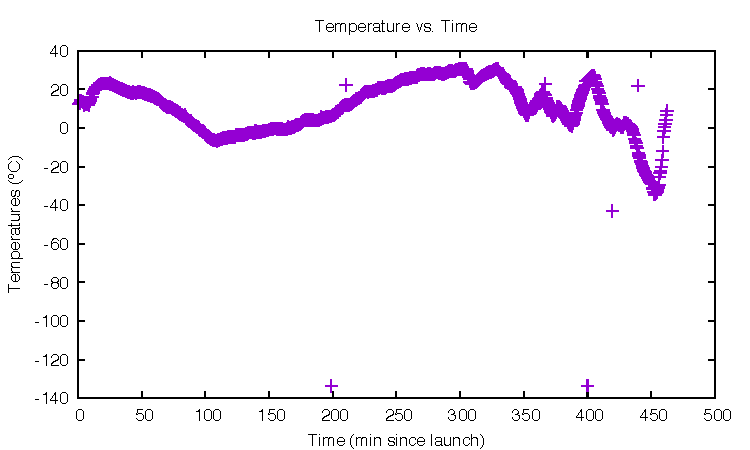
\includegraphics{./tracksoar/temp-time}
\par\end{centering}
\caption{}
\label{ts:temp-time}
\end{figure}


\end{document}
